\documentclass[tikz]{standalone}
\usepackage{amsmath}
\usepackage{pgfplots}
\pgfplotsset{compat=1.16}
\pgfplotsset{
    no markers,
    axis lines=middle,
    xtick={\empty},
    ytick={\empty},
    every axis/.style={
        scale only axis,
        unit vector ratio*=1 1 1,
    },
    every axis plot/.append style={ultra thick},
    xlabel style={at={(ticklabel* cs:1)}, anchor=north west},
    ylabel style={at={(ticklabel* cs:1)}, anchor=east},
}

\def\vgamma{0.75}
\def\vt{.3}
\def\kuno{20}
\def\kdue{0.05}

\begin{document}
    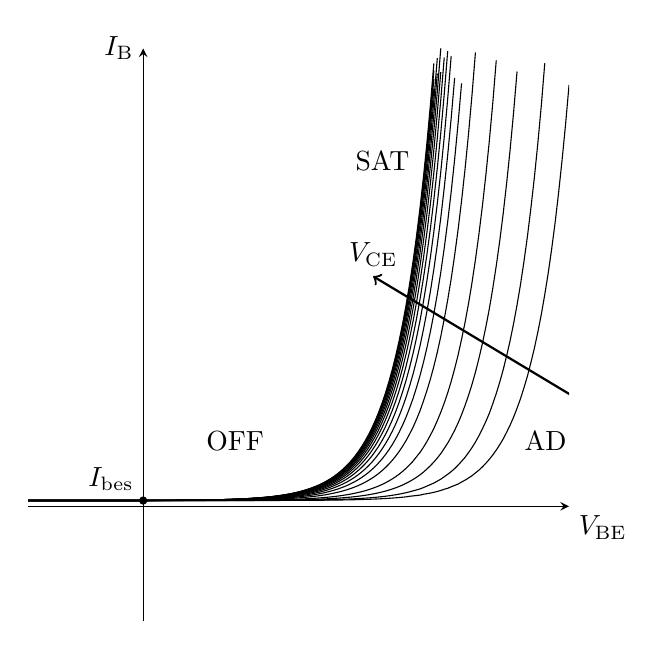
\begin{tikzpicture}[declare function={
            ib(\vbe,\vce) = \kuno *(e^(\vbe/\vt)-1) - (\kuno + \kdue) *(e^((\vbe - \vce)/\vt) -1);
        }]

        \begin{axis}[
                restrict y to domain=-1:4,
                ymin=-1,
                xmin=-1,
                xlabel=$V_\text{BE}$,
                ylabel=$I_\text{B}$,
            ]
            \foreach \i in {
                0.006,
                0.012,
                0.026,
                0.05,
                0.10,..., 0.8}{
                \addplot [
                    thin,
                    domain=-1:5,
                    samples=200,
                    restrict y to domain=-1:4]{ib(x -3, \i)};
            }

            \draw[->, thick] (4.5, 0.5) -- (2, 2) node[above]{$V_\text{CE}$};
            \draw
                (0.8, 0.4) node[above]{OFF}
                (3.5, 0.4) node[above] {AD}
                (2.4, 3) node[left]{SAT}
                (0, \kdue) node[circle, minimum size=3pt, inner sep=0pt, fill=black]{}
                           node[anchor=south east]{$I_\text{bes}$}
                ;
        \end{axis}
    \end{tikzpicture}
\end{document}
